\section{Analysis of the retrieval system}

To implement the ``scan to search'' 3D retrieval system, the most important part is the computation of spherical harmonics. But before that,several pre-processing steps are required. 

Firstly, the scanning noise should be reduced. Therefore before any other processing, the 3D model needs to be put into an appropriate denoising module. Secondly, normalization and rasterization of the model are essential. Normalization can make sure the final matching algorithm will not be affected by the scale of the model. Besides, the influence of outliers will also be reduced. Moreover, rasterization can filter out high frequency noise, and meanwhile keep the granularity of the 3D shape. 

Afterwards, the main retrieval steps can be carried out. Spherical harmonics transformation and distance histogram are able to compute for the pre-processed model. At the first time to use this system, the descriptors' database should be initialized. Following these steps(normalization, rasterization and computation of descriptors), the descriptors' database is able to be generated. And the system is ready for retrieval. To overcome the potential inaccuracy of the results, the system will show six candidates model with high similarities to the input model.

Apart from implementing the main retrieval steps, in the early stage, verification of the algorithms is vital. When the retrieval system is completed, some test cases are also important to evaluate the performance of the system. There are several steps to verify the system: 

\begin{enumerate}[1.]
\item Input a model from the model database; try to find exact the same model
\item Input a model from the model database; rotate the model and try to find the model with the same or similar shape
\item Input a model from the model database; add noise/denoise and try to find the model with same/similar shape
\item Input a scanned model; denoise and try to find the model with same/similar shape
\item Increase the size of the database, and then input a scanned model; denoise and try to find the model with same/similar shape
\end{enumerate}

In the early stage, testing and verification of the algorithms are vital. While the retrieval system is completed, some test cases are also important to evaluate the performance of the system. There are several test cases: 

\begin{enumerate}[1.]
\item Retrieval test
\item Rotation invariant test
\item Noise resistant test
\item ``Scan to search'' test
\item Large database test
\end{enumerate}

The first step is to verify the matching algorithm has no error. The query result is expected to show the model which is exact the same as the input model from the model database. The second step is to verify the rotation invariant of the descriptors. The best result is finding out exact the same model from the database. However, due to the potential error of coefficients in rotation as well as rasterization, if the system shows similar shape, it can be still decided as robust. The third step is to verify the noise resistant property of the system. Because the denoise module as well as the rasterization step cannot perfectly eliminate the noise, the system can be decided as robust if the result shows same or similar shapes. After all these steps, the scanned model can be input to retrieve and test how well the matching algorithm works. The last step is to verify the system's robustness to large database, where a large number of descriptors may have influence to the retrieval accuracy. 

\section{System design}

The flowchart for the pre-processing is in Figure~\ref{scan2search_preprocessing}. It can be noticed that the simulators for rotation and noise are added. In the early stage, in order to verify the rotational invariance property of the descriptors, as well as robustness to random noise, these simulators are essential. But in the final testing of ``scan to search'', these simulators should not be applied to the scanned model. Besides, the judgment step that whether the model is noisy, and the further denoising step depend on the user. 

\begin{figure}[h]
\centering
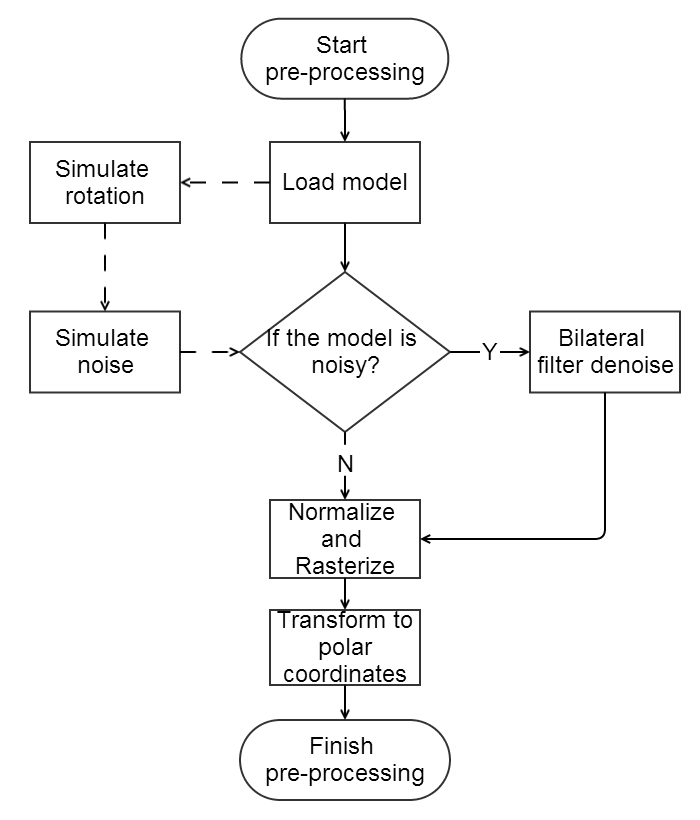
\includegraphics[width=0.8\linewidth]{scan2search_preprocessing}
\caption{Pre-processing of the input model} \label{scan2search_preprocessing}
\end{figure}

The flowchart for the main retrieving process is in Figure~\ref{scan2search_main}. If it is the first time to use the retrieval system, the database for the descriptors should be created. A batch descriptors transformation is required. Every model in the model database will be put into the system, and with the pre-processing steps and spherical harmonics/distance histogram computation, the descriptors database can be generated. With the descriptors' database, and the new descriptors for the input model, the system will compute the similarities between input data and database data. The similarity is simply the Euclidean distance between
descriptors. Besides, since there are two descriptors (spherical harmonics and distance histogram), the result similarities for each of the descriptors will be normalized and combined with weights, which is normally set as 0.5. That is to say, normally the two descriptors are considered to have same weight on the final similarity.

\begin{figure}[h]
\centering
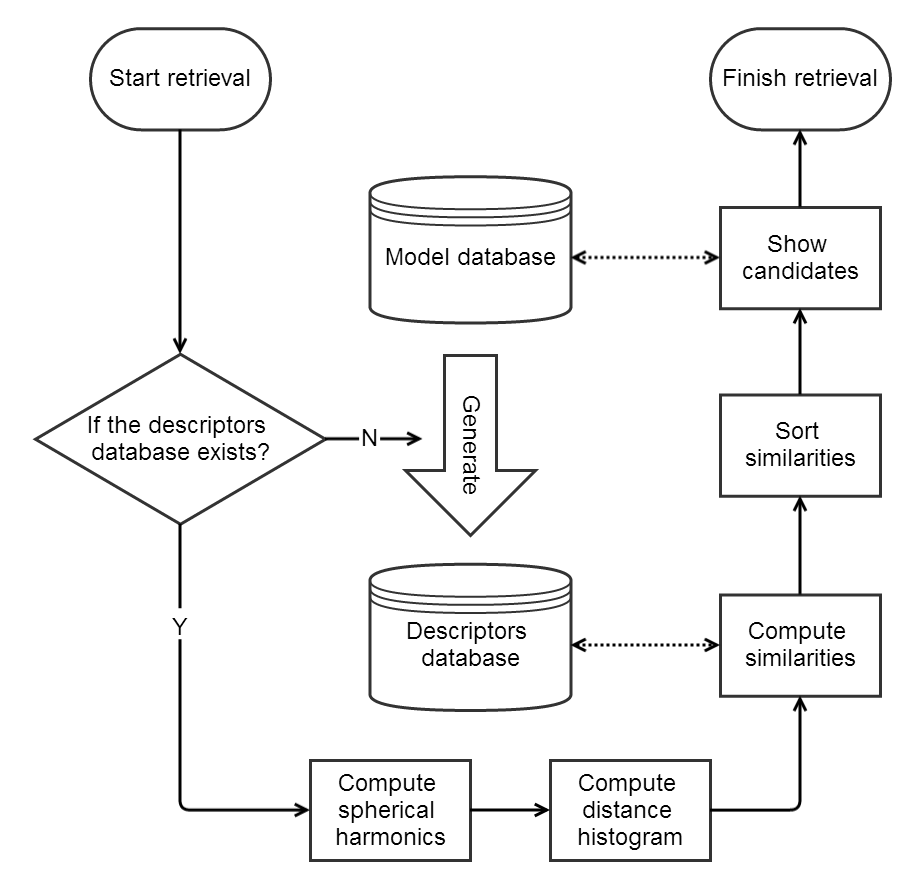
\includegraphics[width=1\linewidth]{scan2search_main}
\caption{Retrieval process} \label{scan2search_main}
\end{figure}

The final user interface for the retrieval system is shown in Figure~\ref{UI}. It can be noticed that each processing step is controlled by relevant button. This design allows manual operations so that to observe the intermediate changes and output on each step. In this way, potential errors can be noticed and avoided. After finishing the testing, the user can choose automatically processing and retrieve.

\begin{figure}[h]
\centering
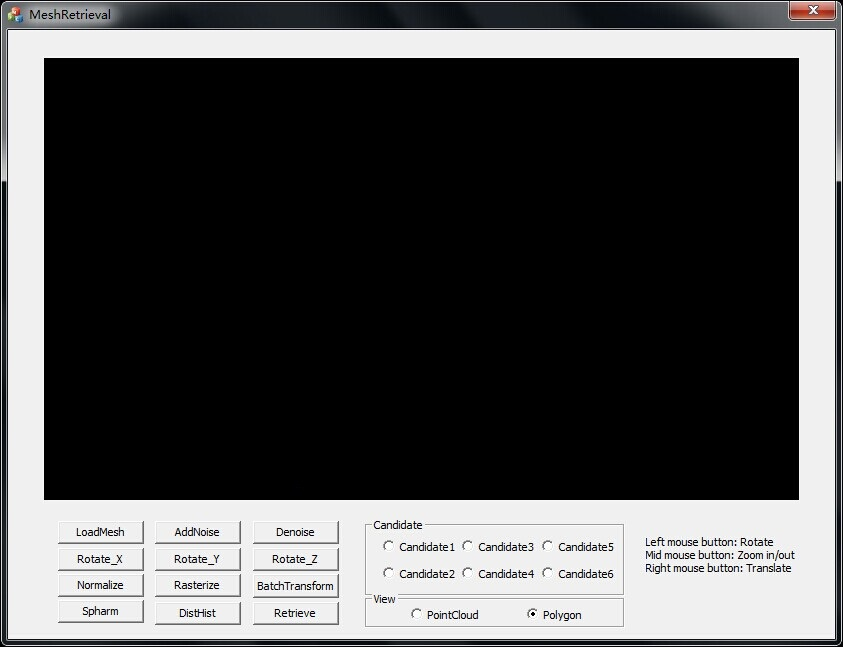
\includegraphics[width=0.7\linewidth]{UI}
\caption{User Interface} \label{UI}
\end{figure}

\section{The final design} \label{sec:thefinaldesign}

At the beginning, there is only one spherical harmonics descriptors applied in the system. However, due to some unknown error in the final descriptors (maybe it is the rasterization error or sampling error in the spherical harmonics transformation), there are sometimes some outliers in the output candidate models, whose shapes are not similar to the input data. For example, with the input model(Figure~\ref{input_initialdesign}), the retrieval result shows six candidates in Figure~\ref{output_initialdesign}. It can be observed that some outlier candidates with unsimilar shapes are demonstrated. 


\begin{figure}[h]
\centering
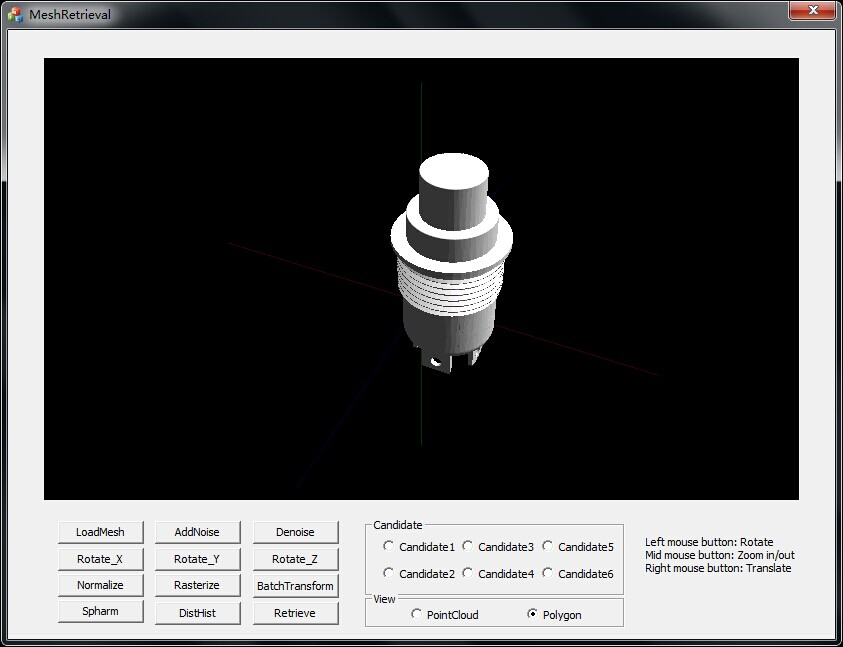
\includegraphics[width=0.7\linewidth]{input_initialdesign}
\caption{Input of the initial design} \label{input_initialdesign}
\end{figure}

\begin{figure}[h]
\centering
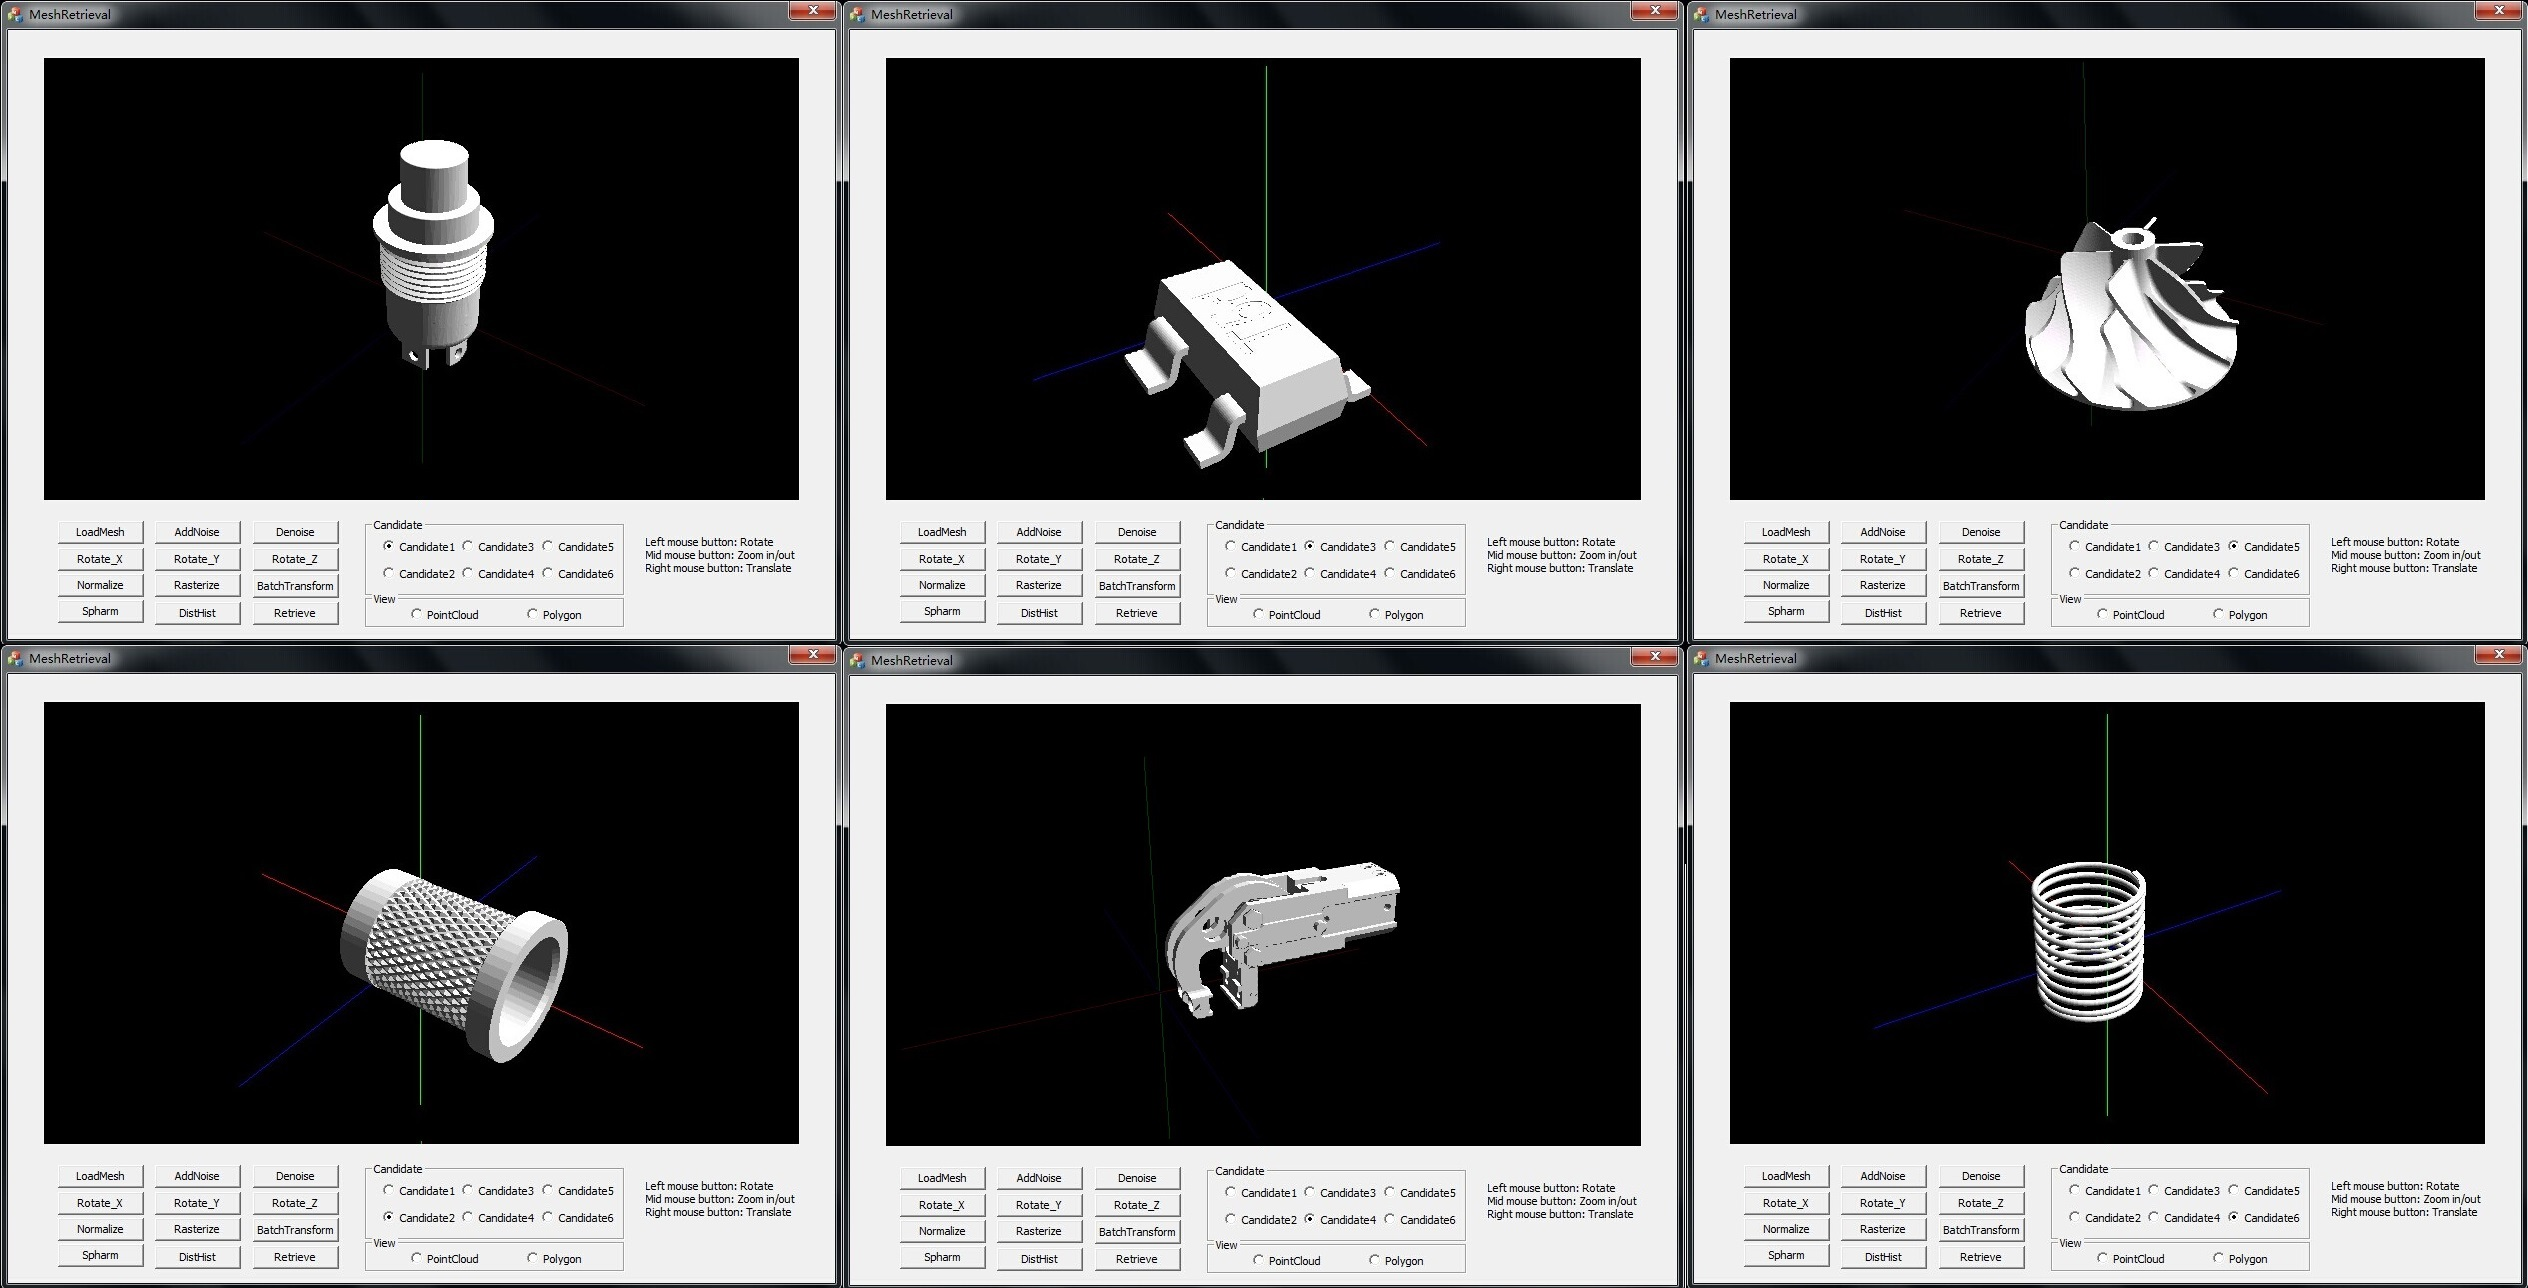
\includegraphics[width=0.7\linewidth]{output_initialdesign}
\caption{Output of the initial design} \label{output_initialdesign}
\end{figure}

Therefore, another simpler distance histogram  descriptors are added. The matching results combine the similarities computed by distance histogram and spherical harmonics, and reduce matching errors. Figure~\ref{output_finaldesign} demonstrates the results of the final design with the same input model.

\begin{figure}[h]
\centering
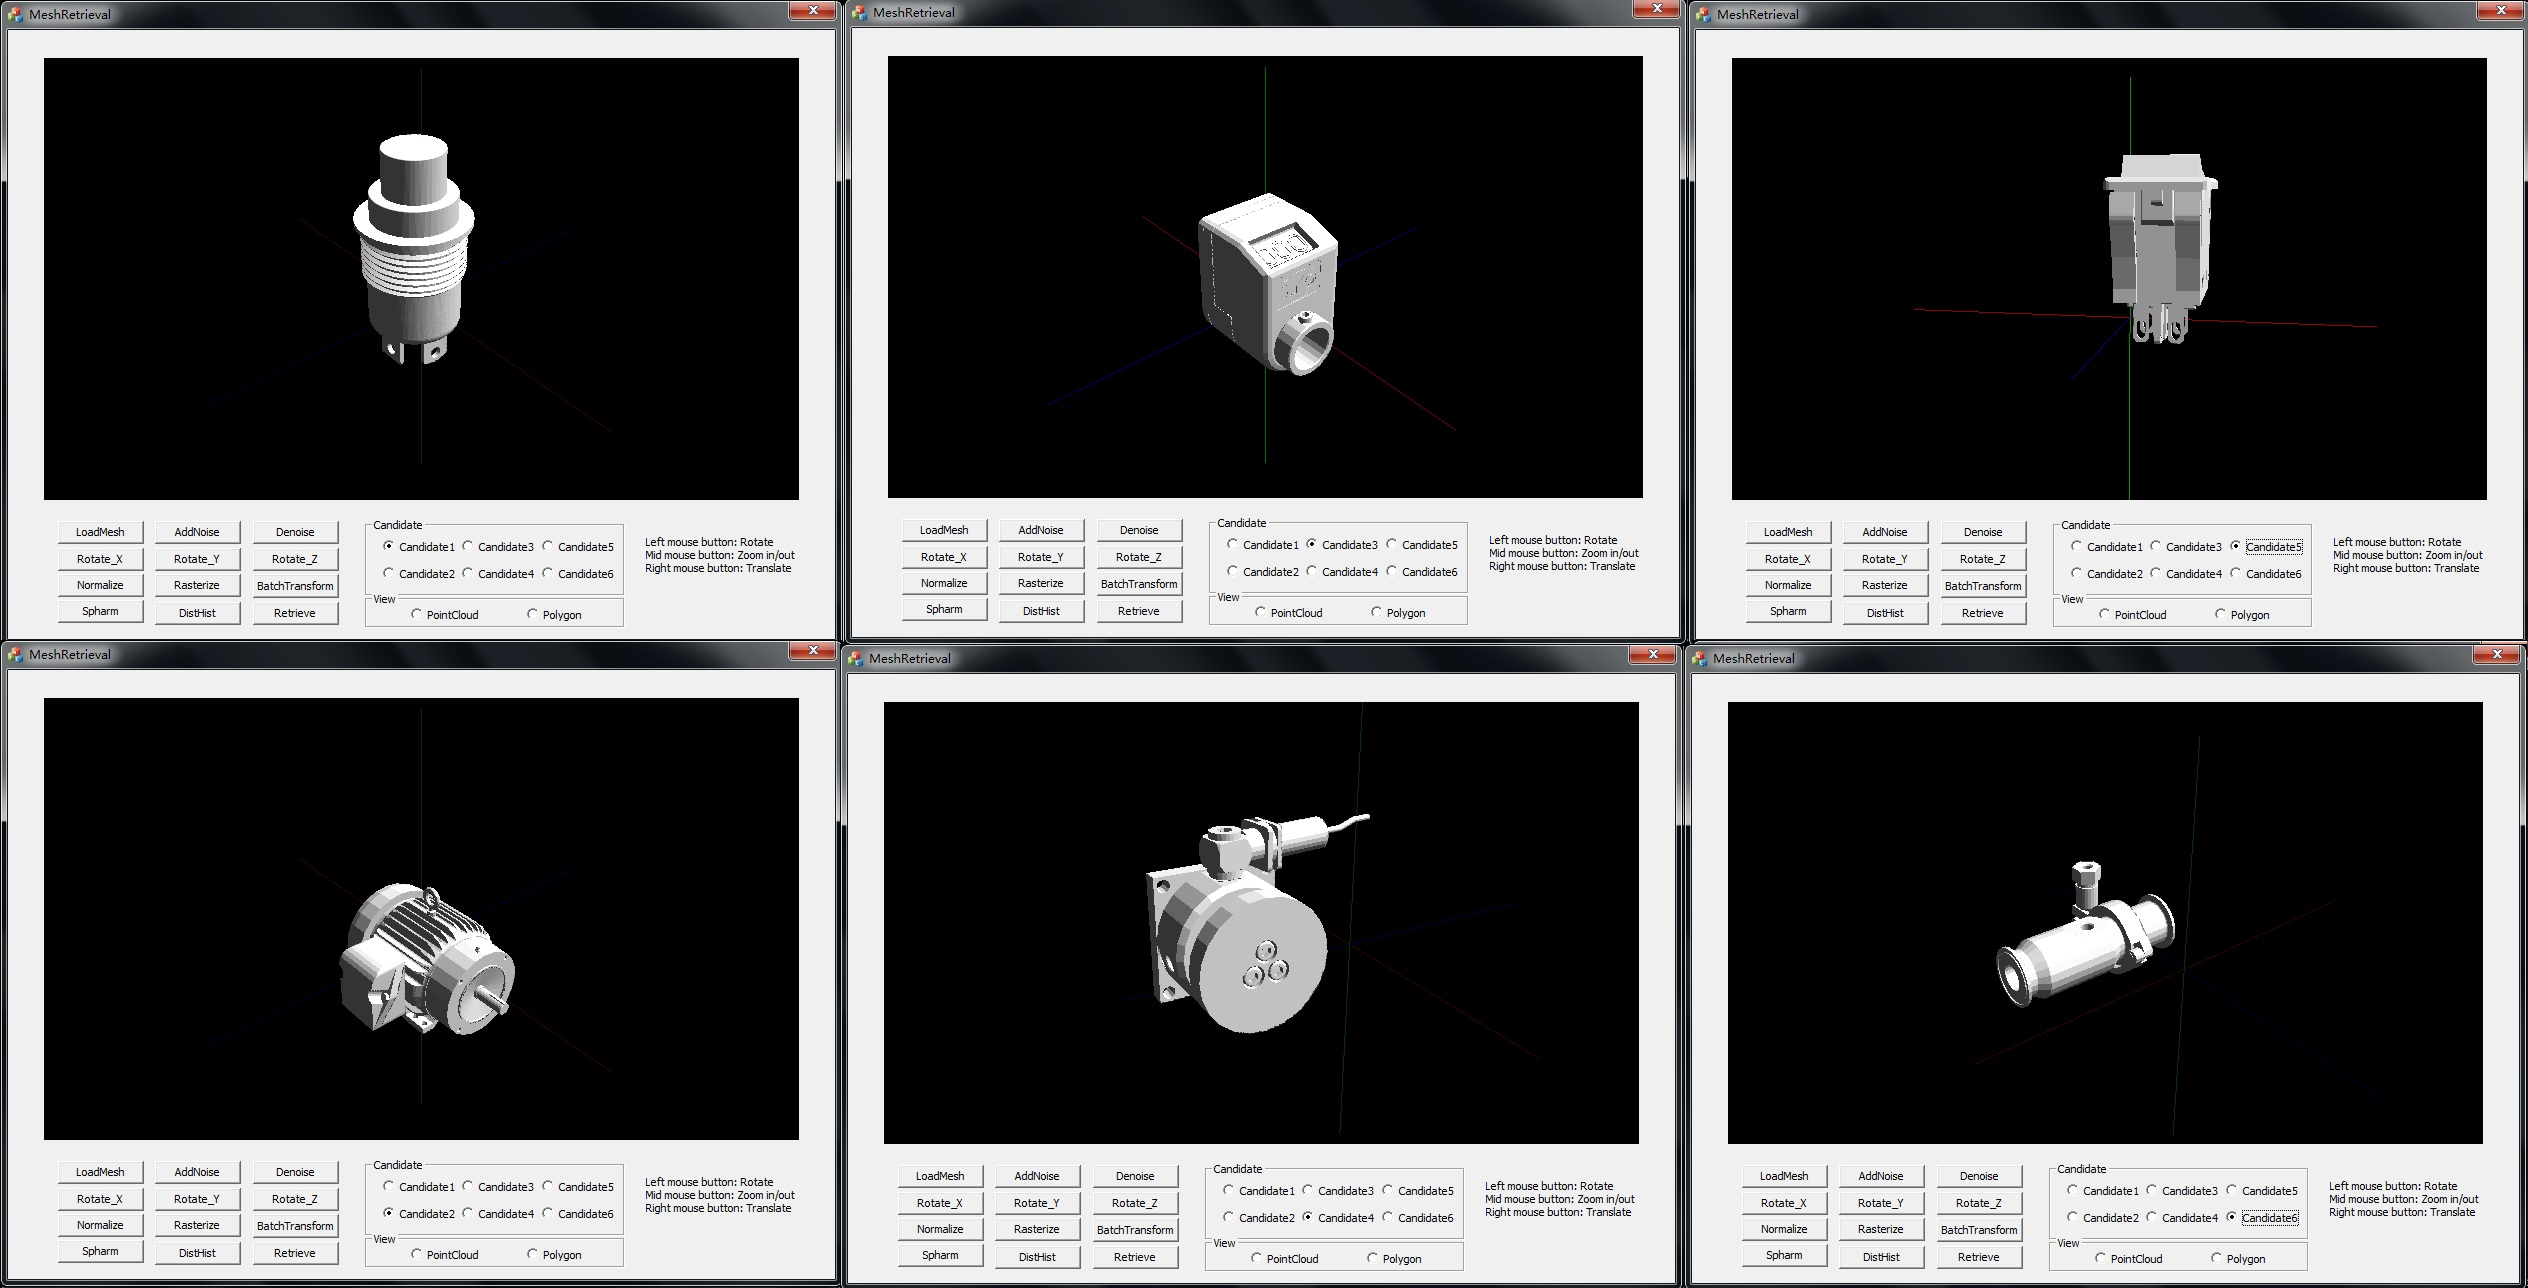
\includegraphics[width=0.7\linewidth]{output_finaldesign}
\caption{Output of the final design} \label{output_finaldesign}
\end{figure}

The verification also worths mentioning. Well designed tests can verify the correctness of the system design and implementation, also they can help to avoid potential risks for further implementation. 

The initial design only has the spherical harmonics descriptors. And spherical harmonics transformation is difficult to implemented. At first the transformation is implemented incorrectly, nevertheless the descriptors can be computed. And even test one ``Retrieval test'' passes. That is because the incorrect descriptors show some features, to some extent. However, the rotational invariance test does not pass, due to the wrong spherical harmonics decomposition. Thus the spherical harmonics decomposition is reimplemented and tested. 
Additionally, after enlarging the database to size 60, the output shows the weakness and inaccuracy of single type of descriptors. Therefore another distance histogram matching algorithm is added for assistance.
